\documentclass[11pt, oneside]{article}   	% use "amsart" instead of "article" for AMSLaTeX format
%\usepackage{geometry}                		% See geometry.pdf to learn the layout options. There are lots.
%\geometry{letterpaper}                   		% ... or a4paper or a5paper or ... 
%\geometry{landscape}                		% Activate for rotated page geometry
%\usepackage[parfill]{parskip}    		% Activate to begin paragraphs with an empty line rather than an indent

\usepackage{geometry}
 \geometry{
 a4paper,
 total={170mm,257mm},
 left=20mm,
 top=25mm,
 bottom=25mm
 }

\usepackage{graphicx}				% Use pdf, png, jpg, or eps§ with pdflatex; use eps in DVI mode
								% TeX will automatically convert eps --> pdf in pdflatex		
\usepackage{amssymb}
\usepackage{amsmath}
\usepackage{fancyhdr}
\usepackage[utf8]{inputenc}
\usepackage[english]{babel}
\usepackage{enumerate}
\usepackage{arcs}
\usepackage{cancel}
\usepackage{xfrac}
\usepackage{amsthm}
\usepackage{gensymb}
\usepackage{xspace}
\usepackage{hyperref}
\usepackage{fancyvrb}
\usepackage{subcaption}
%\usepackage{fontawesome}


\usepackage{listings}
\usepackage[most]{tcolorbox}
%\usepackage{inconsolata}

\newtcblisting[auto counter]{sexylisting}[2][]{sharp corners, 
    fonttitle=\bfseries, colframe=gray, listing only, 
    listing options={basicstyle=\ttfamily,language=java}, 
    title=Listing \thetcbcounter: #2, #1}

%\usepackage{ctex}

%SetFonts

%SetFonts

\usepackage[inline]{asymptote}


\usepackage[framemethod=tikz]{mdframed}

\newtheorem{example}{Example}
\mdfdefinestyle{examp}{
  linecolor=cyan,
  backgroundcolor=yellow!20
  % , rotatebox
}
\surroundwithmdframed[style=examp]{example}

\usepackage{environ}
\NewEnviron{Example}
{%
\noindent
\begin{minipage}[t]{\linewidth}
\begin{example}
\BODY
\end{example}%
\end{minipage}%
}%

\newtheorem*{solution}{Solution}
\mdfdefinestyle{sol}{
  linecolor=red,
  % , rotatebox
}
\surroundwithmdframed[style=sol]{solution}

\usepackage{environ}
\NewEnviron{Solution}
{%
\noindent
\begin{minipage}[t]{\linewidth}
\begin{solution}
\BODY
\end{solution}%
\end{minipage}%
}%


\pagestyle{fancy}
\fancyhf{}
\lhead{\leftmark}
\cfoot{\thepage}

\title{Assignment 2: Camera Calibration}
\author{Zifei (David) Zhong}
\date{CSCE 774, Fall 2023}							% Activate to display a given date or no date

\newcommand{\latex}{\LaTeX\xspace}


\begin{document}
\maketitle

\section{Using the Kalibr Package}
With Ubuntu 20.04 operating system, I installed ROS noetic and Docker 24.0.7.

\subsection{Docker Installation}
It took me a while to get Docker running properly. I mostly followed the installation instructions from the Docker project website. The following is my docker information
\begin{verbatim}
>>>  docker version
Client: Docker Engine - Community
 Cloud integration: v1.0.35+desktop.5
 Version:           24.0.7
 API version:       1.41 (downgraded from 1.43)
 Go version:        go1.20.10
 Git commit:        afdd53b
 Built:             Thu Oct 26 09:08:01 2023
 OS/Arch:           linux/amd64
 Context:           default

Server:
 Engine:
  Version:          20.10.24
  API version:      1.41 (minimum version 1.12)
  Go version:       go1.20.7
  Git commit:       5d6db84
  Built:            Wed Aug 23 20:55:00 2023
  OS/Arch:          linux/amd64
  Experimental:     false
 containerd:
  Version:          v1.6.20
  GitCommit:        2806fc1057397dbaeefbea0e4e17bddfbd388f38
 runc:
  Version:          1.1.5
  GitCommit:        
 docker-init:
  Version:          0.19.0
  GitCommit:        de40ad0

\end{verbatim}

\subsection{Troubleshooting}
Once the Docker is installed, the communication might not work properly. In my case, I kept getting the following error message while running \verb+kalibr+:
\begin{verbatim}
...
_tkinter.TclError: couldn't connect to display ":0" 
\end{verbatim}

After searching on Google and trying different patches for several hours, I finally got the right solution by asking ChatGPT: adding the \verb+--net=host+ arguments to the command \verb+docker run+
\begin{verbatim}
docker run -it --net=host -e "DISPLAY" -e "QT_X11_NO_MITSHM=1" \
           -v "/tmp/.X11-unix:/tmp/.X11-unix:rw" \
           -v "$FOLDER:/data" kalibr
\end{verbatim}

\subsection{Generating Reports}
Run the following command for the three ROS bag files provided, I got three reports generated. 
\begin{verbatim}
rosrun kalibr kalibr_calibrate_cameras --bag /data/GX010181.bag \
              --target /data/aprilgrid_5x7Canvas.yml \
              --models pinhole-radtan \
              --topics /gopro/image_raw/compressed
\end{verbatim}

One example report is illustrated in Figure~\ref{fig.1}, which is the result of generated using ROS bag file GX010181.bag. The results include camera distortion and projection parameters, polar errors, azimuthal errors, reprojection errors, and location of removed outlier corners. The other two reports are similar.

\begin{figure}[ht]
\centering
\begin{subfigure}[b]{0.3\textwidth}
\includegraphics[width=\textwidth]{imgs/kalibr1.png}
\caption{Parameters}
\end{subfigure}
\begin{subfigure}[b]{0.3\textwidth}
\includegraphics[width=\textwidth]{imgs/kalibr2.png}
\caption{Estimated Poses}
\end{subfigure}
\begin{subfigure}[b]{0.3\textwidth}
\includegraphics[width=\textwidth]{imgs/kalibr3.png}
\caption{Polar Error}
\end{subfigure}\\
\begin{subfigure}[b]{0.3\textwidth}
\includegraphics[width=\textwidth]{imgs/kalibr4.png}
\caption{Azimuthal Error}
\end{subfigure}
\begin{subfigure}[b]{0.3\textwidth}
\includegraphics[width=\textwidth]{imgs/kalibr5.png}
\caption{Reprojection Errors}
\end{subfigure}
\begin{subfigure}[b]{0.3\textwidth}
\includegraphics[width=\textwidth]{imgs/kalibr6.png}
\caption{Removed outlier corners}
\end{subfigure}

\caption{Results generated by kalibr with bag file GX010181.bag}
\label{fig.1}
\end{figure}

\newpage
\section{Performing Camera Calibration Online}
In the part, I utilized the ROS camera calibration package to calibrate a Logi HD 1080P camera attached to my Ubuntu 20.04 system. The setup was pretty straightforward. Running ROS node \verb+usb_cam+ and I quickly saw the images from ROS topic \verb+/usb_cam/image_raw+.

\subsection{Troubleshooting}
The pain came from the fact that I ran the calibration via 
\begin{verbatim}
rosrun camera_calibration cameracalibrator.py --size 6x8 \
    --square 0.031 image:=/usb_cam/image_raw camera:=/usb_cam
\end{verbatim}

With the above running, I moved the black-white grid board in front of the camera for 10 minutes, for many times, nothing came out. It took me almost a day to find out that I should change the parameter \verb+--size 6x8+ to \verb+--size 4x6+. 

Basically, the calibrator seemed not be able to recognize the whole black-white grid, it only recognize inner subgrids, which should have smaller size than \verb+6x8+.

\subsection{Calibrating Process}
The calibrating process basically involves moving the black-white grid in front of the camera, placing the grid from different angles, and different distance, so that the calibrator can collect enough data for calibration. Once the calibrator collects a frame of data, it displays some colorful lines on camera image, as show in Figure~\ref{fig.2.a}. Once the calibrator captures enough samples, as shown in Figure~\ref{fig.2.b}, it starts to generate calibration results.

\begin{figure}[ht]
\centering
\begin{subfigure}[b]{0.4\textwidth}
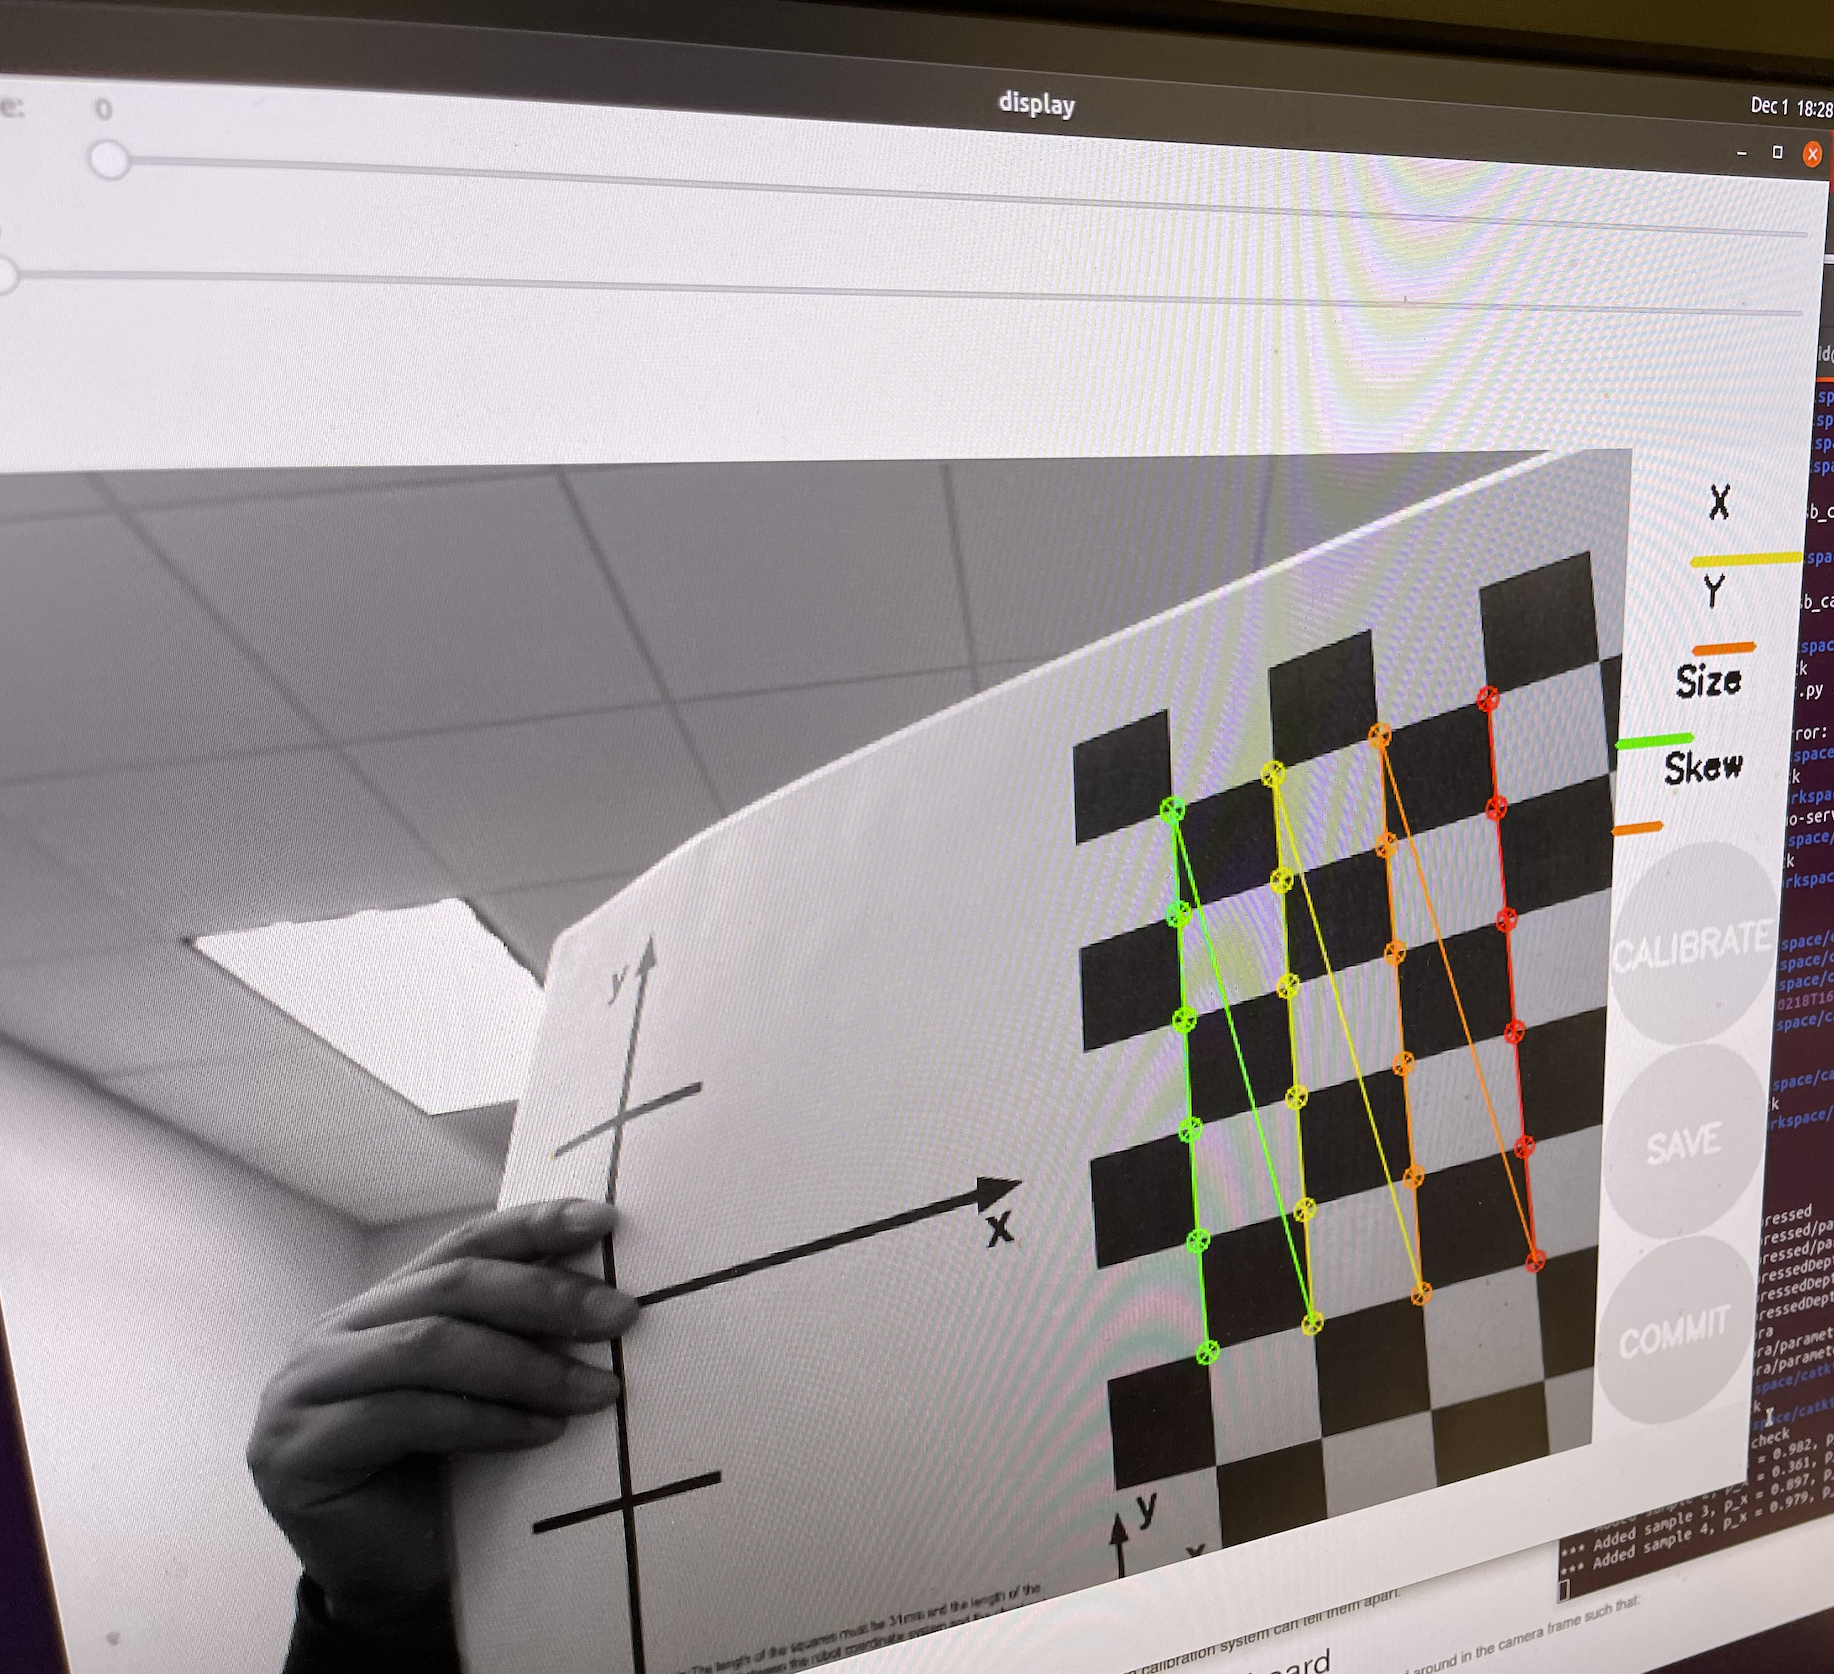
\includegraphics[width=\textwidth]{imgs/calibration1.png}
\caption{Captures a sample frame}
\label{fig.2.a}
\end{subfigure}
\begin{subfigure}[b]{0.455\textwidth}
\includegraphics[width=\textwidth]{imgs/calibration2.png}
\caption{All samples captured }
\label{fig.2.b}
\end{subfigure}
\caption{Online Calibration}
\label{fig.2}
\end{figure}

\subsection{Calibration Results}
Finally, the calibration data were written to file \verb+head_camera.yaml+:
\begin{verbatim}
D = [0.009249503266722884, -0.028967392445748585, 0.014480091428682588,
       -0.005780678000630155, 0.0]
K = [621.8880241657102, 0.0, 310.214997181103, 0.0, 625.439049296969, 
        268.8064508603691, 0.0, 0.0, 1.0]
R = [1.0, 0.0, 0.0, 0.0, 1.0, 0.0, 0.0, 0.0, 1.0]
P = [626.0367431640625, 0.0, 306.4703511162297, 0.0, 0.0, 625.990478515625, 
        273.8179633314576, 0.0, 0.0, 0.0, 1.0, 0.0]
# oST version 5.0 parameters

[image]

width
640

height
480

[narrow_stereo]

camera matrix
621.888024 0.000000 310.214997
0.000000 625.439049 268.806451
0.000000 0.000000 1.000000

distortion
0.009250 -0.028967 0.014480 -0.005781 0.000000

rectification
1.000000 0.000000 0.000000
0.000000 1.000000 0.000000
0.000000 0.000000 1.000000

projection
626.036743 0.000000 306.470351 0.000000
0.000000 625.990479 273.817963 0.000000
0.000000 0.000000 1.000000 0.000000
\end{verbatim}
\end{document} 
